% File: chapters/chapter3.tex
% Chapter 3: System Design and Architecture
% Include this in your main document with \include{chapters/chapter3}
% Ensure you have booktabs, array, enumitem, and graphicx in preamble.

\chapter{System Design and Architecture}

\section{Overview}

The Fleet Management System is built on a distributed microservices architecture designed for intelligent vehicle dispatch, real-time GPS tracking, and automated fault management. The system consists of four primary components working together to provide a comprehensive fleet management solution with AI-powered decision-making capabilities.

\subsection{System Components}

The system is composed of the following main components:

\begin{enumerate}
    \item \textbf{Frontend Application} (React/TypeScript) -- User interface and real-time visualization
    \item \textbf{Backend Service} (Node.js/Express) -- Core business logic and API gateway
    \item \textbf{ML Service} (Python/FastAPI) -- Machine learning dispatch predictions
    \item \textbf{Vehicle Simulator} (Node.js) -- Hardware device simulation for testing
\end{enumerate}

\section{Overall System Architecture}

\subsection{High-Level Architecture Diagram}

\begin{figure}[h]
    \centering
    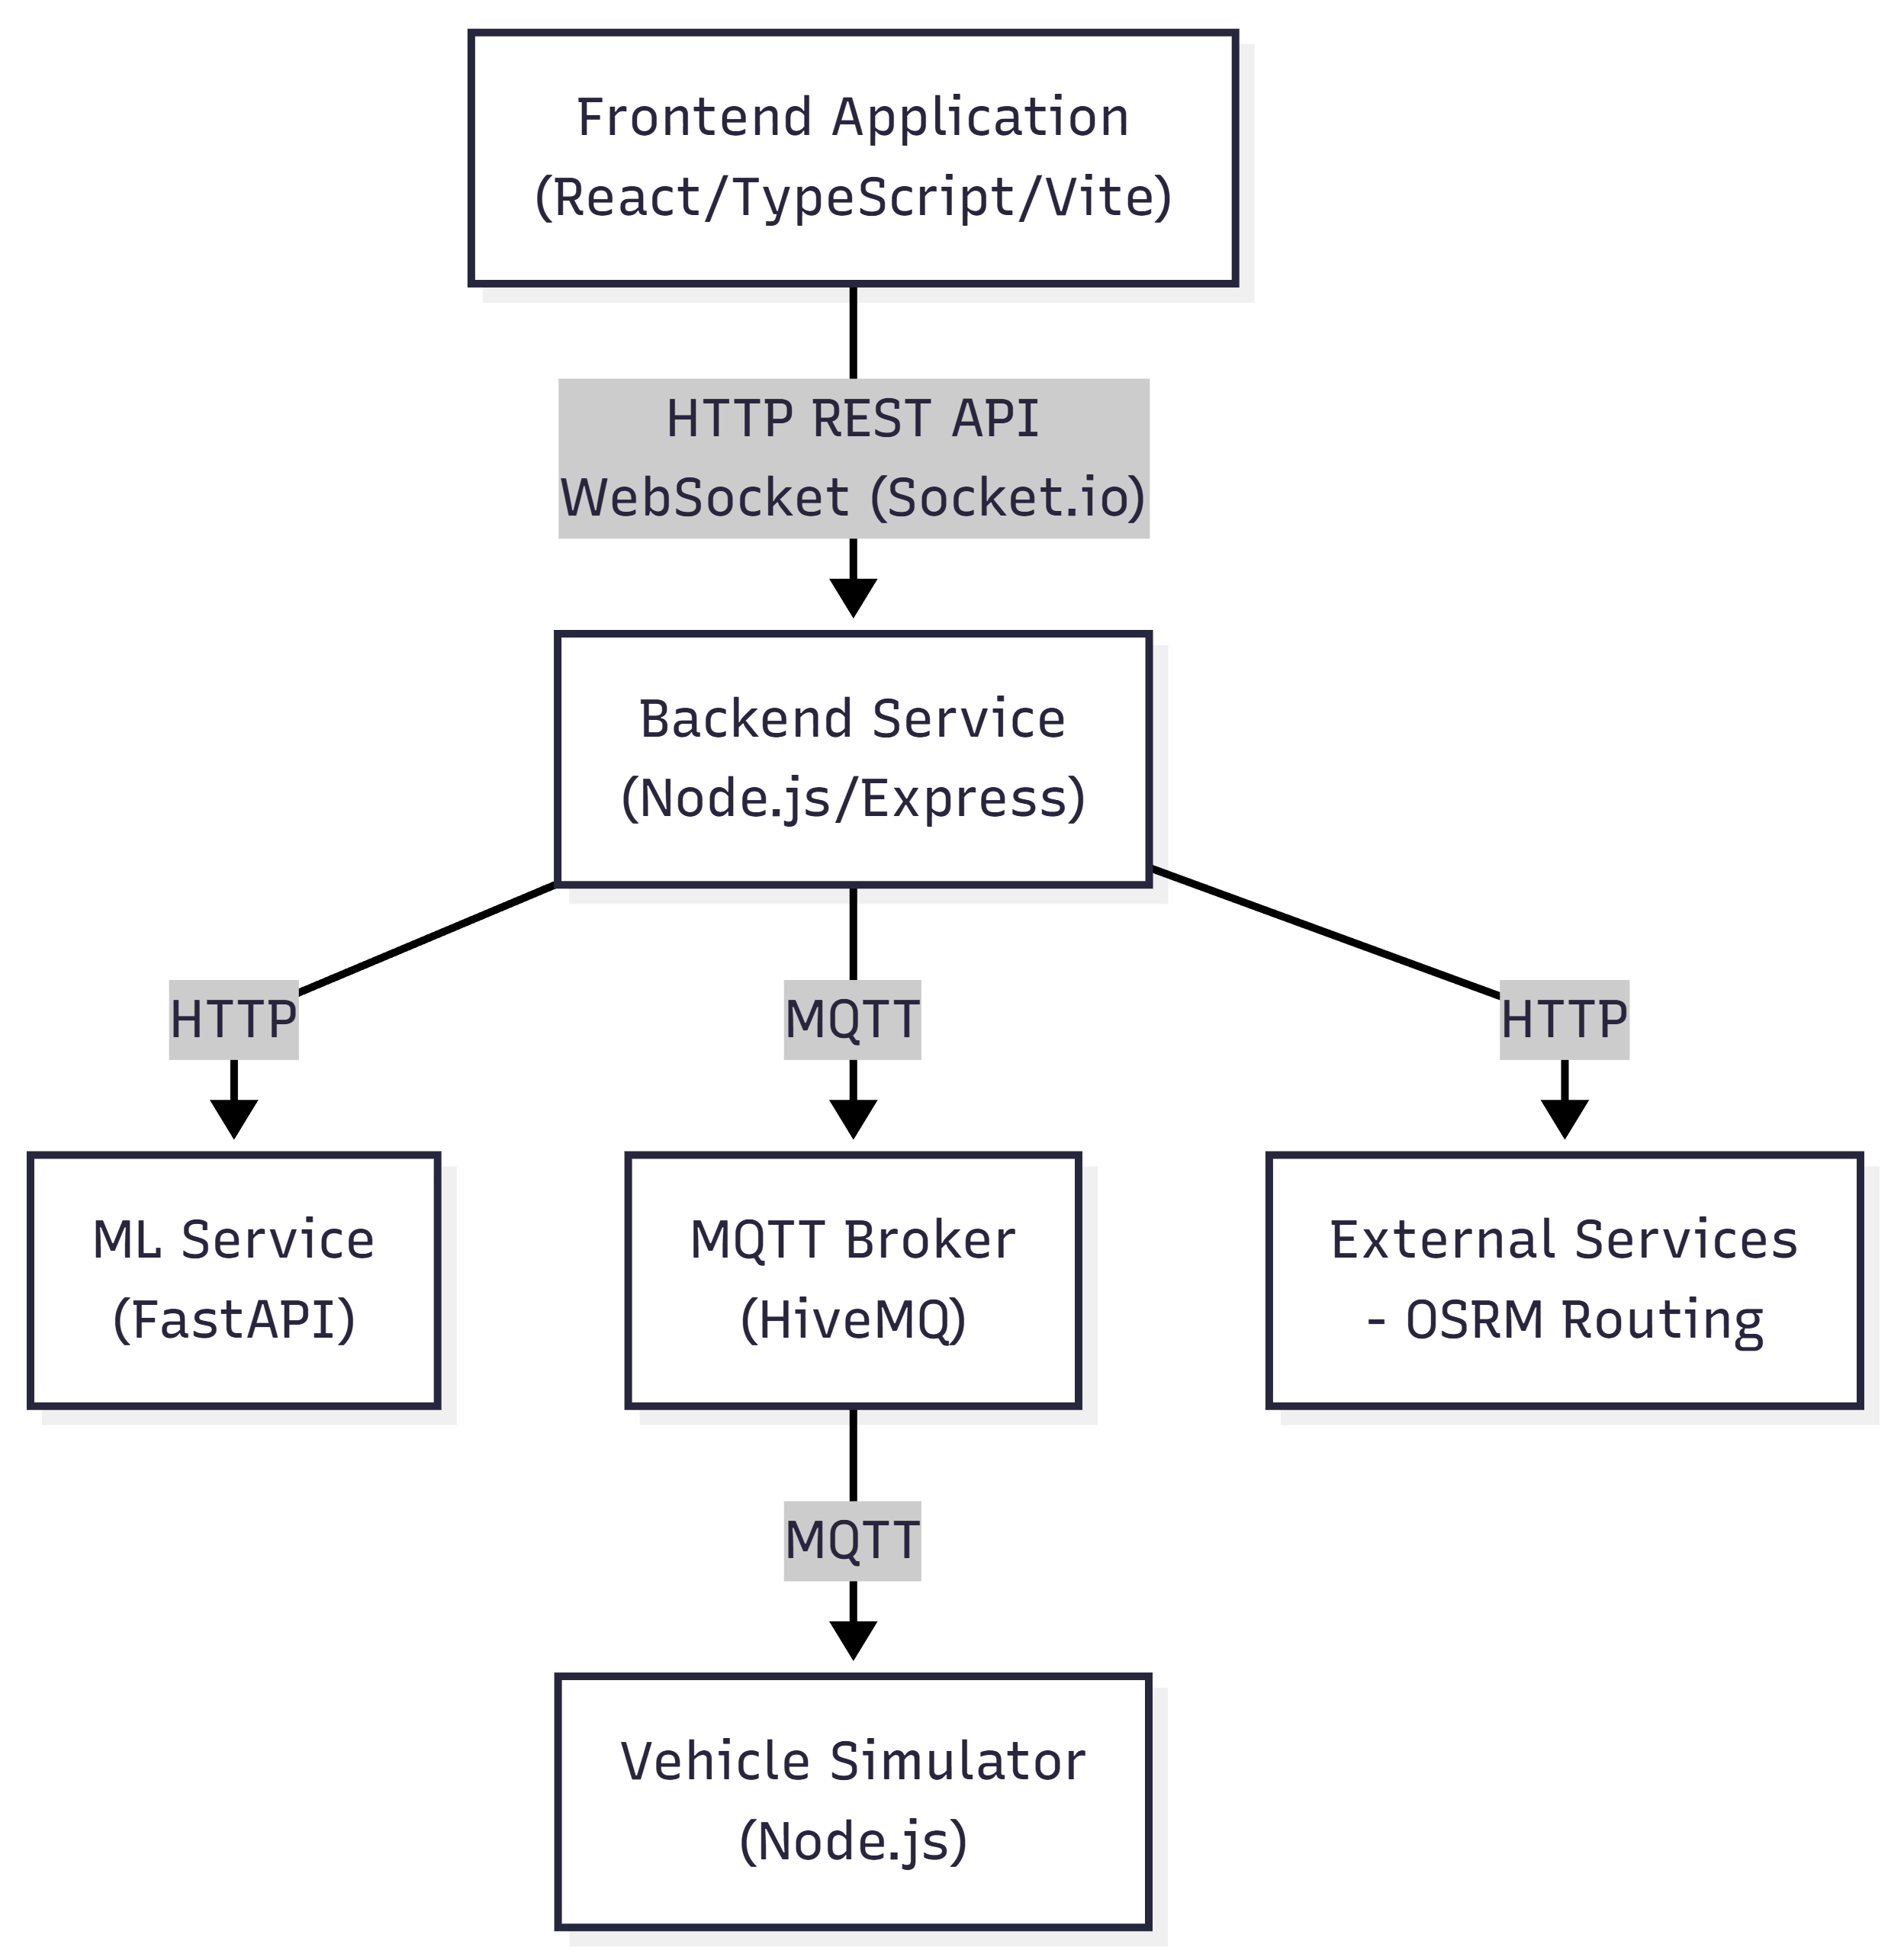
\includegraphics[width=0.95\textwidth]{chapter3/figs/3.1.png} % Replace with your actual image path
    \caption{High-Level Architecture Diagram}
    \label{fig:3.1}
\end{figure}

\section{Frontend Application}

The frontend is a modern single-page application built with React and TypeScript, providing an intuitive interface for fleet management.

\subsection{Key Technologies}

\begin{itemize}
    \item Framework: React 18
    \item Language: TypeScript
    \item Build Tool: Vite
    \item State Management: React Context API + TanStack Query
    \item UI Library: Tailwind CSS + shadcn/ui
    \item Maps: MapLibre GL JS
    \item Real-time: Socket.io Client
\end{itemize}

\subsection{Frontend Components}

The frontend is organized into modular components:

\begin{itemize}
    \item \textbf{Dashboard}: Main control panel with real-time updates
    \item \textbf{MapView}: Interactive map with vehicle markers and routes
    \item \textbf{FleetList}: Vehicle status and management panel
    \item \textbf{DispatchPanel}: Fault management and dispatch interface
    \item \textbf{AlertSystem}: Real-time notification handler
    \item \textbf{Auth Components}: Login and access control
\end{itemize}

\subsection{Frontend Architecture}

\begin{itemize}
    \item Component-based architecture
    \item Custom hooks for API interactions
    \item Global state management for shared data
    \item Responsive design for desktop/mobile
    \item Dark/Light mode support
\end{itemize}

\subsection{Data Flow in Frontend}

\begin{enumerate}
    \item API calls via TanStack Query for data fetching
    \item WebSocket events for real-time updates
    \item Context providers for global state
    \item Local storage for user preferences
\end{enumerate}

\section{Backend Service}

The backend serves as the central orchestration layer, handling business logic, database interactions, and integration with other services.

\subsection{Key Technologies}

\begin{itemize}
    \item Runtime: Node.js 20
    \item Framework: Express.js
    \item Database: MongoDB with Mongoose
    \item Real-time: Socket.io
    \item Cache: Node-cache
    \item Logging: Winston
    \item Validation: Joi
\end{itemize}

\subsection{Backend Structure}

\begin{itemize}
    \item \textbf{Routes/Controllers}: API endpoints organization
    \item \textbf{Services}: Business logic modules
    \item \textbf{Models}: Database schemas
    \item \textbf{Middleware}: Authentication, error handling
    \item \textbf{Utils}: Helper functions
\end{itemize}

\subsection{Key Backend Features}

\begin{itemize}
    \item RESTful API with JWT authentication
    \item Real-time WebSocket server
    \item AI-powered dispatch engine
    \item GPS tracking and route calculation
    \item Fault management workflow
    \item Vehicle and trip tracking
\end{itemize}

\subsection{Backend Data Models}

\begin{itemize}
    \item User/Driver schemas with roles
    \item Vehicle with status and location
    \item Fault with priority and assignment
    \item Trip with start/end metrics
    \item GPS points with timestamps
\end{itemize}

\section{ML Service}

The ML service provides intelligent dispatch recommendations using machine learning models.

\subsection{Key Technologies}

\begin{itemize}
    \item Framework: FastAPI
    \item ML Library: scikit-learn
    \item Data Processing: pandas, numpy
    \item Model Persistence: joblib
\end{itemize}

\subsection{ML Service Structure}

\begin{itemize}
    \item API endpoints for prediction/training
    \item Model loading and caching
    \item Feature validation
    \item Training pipeline
    \item Health monitoring
\end{itemize}

\subsection{Model Details}

\begin{itemize}
    \item Type: RandomForestRegressor
    \item Features: Distance, performance, fatigue, etc.
    \item Training: Synthetic data with rule-based targets
    \item Prediction: Batch scoring for candidates
\end{itemize}

\subsection{ML Integration}

\begin{itemize}
    \item REST API calls from backend
    \item Fallback to rule-based if unavailable
    \item On-demand model training
    \item Performance metrics tracking
\end{itemize}

\section{Vehicle Simulator}

The simulator emulates hardware devices for development and testing.

\subsection{Key Technologies}

\begin{itemize}
    \item Runtime: Node.js
    \item HTTP Client: Axios
    \item MQTT Client: mqtt.js
    \item Routing: OSRM API with Haversine fallback
\end{itemize}

\subsection{Simulator Components}

\begin{itemize}
    \item Vehicle state management
    \item Route calculation
    \item GPS movement simulation
    \item Dispatch polling
    \item Work completion timer
\end{itemize}

\subsection{Simulation Features}

\begin{itemize}
    \item Multiple vehicle support
    \item Real-time GPS publishing
    \item Automatic status updates
    \item Route following with waypoints
    \item MQTT and API integration
\end{itemize}

\subsection{Simulator Workflow}

\begin{itemize}
    \item Poll for dispatches
    \item Calculate and follow routes
    \item Send periodic GPS updates
    \item Simulate arrival and work
    \item Reset after completion
\end{itemize}

\section{System Integration Details}

\subsection{Frontend-Backend Integration}

\begin{itemize}
    \item REST API for data operations
    \item WebSocket for real-time events
    \item JWT authentication
    \item Query caching with TanStack
\end{itemize}

\subsection{Backend-ML Service Integration}

\begin{itemize}
    \item HTTP REST API calls
    \item Health check before prediction
    \item Feature extraction in backend
    \item Fallback rule-based dispatch
\end{itemize}

\subsection{Backend-Simulator Integration}

\begin{itemize}
    \item REST API for status/GPS
    \item MQTT for alerts/confirmations
    \item Polling for dispatch detection
    \item Real-time GPS streaming
\end{itemize}

\subsection{Backend-External Services Integration}

\subsubsection{OSRM Routing Service}

\textbf{Communication Protocol}: HTTP REST API

\textbf{Integration Strategy}:
\begin{itemize}
    \item Circuit breaker pattern for resilience
    \item Automatic fallback to Haversine distance calculation
    \item Route caching (5-minute TTL) to reduce API calls
    \item Consistent coordinate format: [latitude, longitude]
\end{itemize}

\textbf{Error Handling}:
\begin{itemize}
    \item Circuit breaker opens after 3 failures
    \item Automatic recovery after 60 seconds
    \item Fallback calculation using Haversine formula
\end{itemize}

\subsubsection{MQTT Broker (HiveMQ Cloud)}

\textbf{Communication Protocol}: MQTT over TLS (mqtts)

\textbf{Integration Strategy}:
\begin{itemize}
    \item Persistent connection with auto-reconnection
    \item Message queuing when disconnected
    \item QoS Level 1 (at least once delivery)
    \item Topic-based message routing
\end{itemize}

\textbf{Topics Structure}:
\begin{itemize}
    \item Subscriptions: \texttt{vehicle/\{vehicle\_number\}/confirmation}, \texttt{vehicle/\{vehicle\_number\}/resolved}
    \item Publications: \texttt{device/\{device\_id\}/dispatch}
\end{itemize}

\subsection{Database Integration}

\textbf{Database}: MongoDB

\textbf{Integration Strategy}:
\begin{itemize}
    \item Mongoose ODM for schema validation
    \item Connection pooling (2--10 connections)
    \item Indexes for performance optimization
    \item Transaction support for atomic operations
\end{itemize}

\textbf{Data Models}:
\begin{itemize}
    \item Vehicle, Fault, Trip, GPS, Route, User, Driver, Alert, HardwareDevice
\end{itemize}

\textbf{Relationships}:
\begin{itemize}
    \item Reference-based relationships (ObjectId references)
    \item Embedded documents for simple nested data
    \item One-to-many and many-to-many relationships
\end{itemize}

\subsection{Container Integration (Docker)}

\textbf{Integration Strategy}:
\begin{itemize}
    \item Docker Compose for multi-container orchestration
    \item Service discovery via container names
    \item Environment variables for configuration
    \item Volume mounts for persistent data
    \item Network isolation and communication
\end{itemize}

\textbf{Container Dependencies}:
\begin{itemize}
    \item Frontend depends on Backend
    \item Backend depends on ML Service
    \item All services connect to MongoDB
    \item Backend connects to MQTT Broker (external)
    \item Backend connects to OSRM (external)
\end{itemize}

\subsection{Authentication and Authorization Integration}

\textbf{Integration Strategy}:
\begin{itemize}
    \item JWT tokens for stateless authentication
    \item Role-based access control (RBAC)
    \item Token storage in frontend (localStorage)
    \item Token validation middleware in backend
    \item Optional authentication for development
\end{itemize}

\textbf{Flow}:
\begin{enumerate}
    \item User logs in via \texttt{/api/auth/login}
    \item Backend validates credentials and generates JWT
    \item Frontend stores token and includes in requests
    \item Backend validates token on protected routes
    \item Role-based permissions enforced at controller level
\end{enumerate}

\section{System Integration Summary}

The system integrates multiple components through well-defined interfaces and communication protocols:

\begin{enumerate}
    \item \textbf{Frontend $\leftrightarrow$ Backend}: REST API and WebSocket for bidirectional communication
    \item \textbf{Backend $\leftrightarrow$ ML Service}: HTTP REST API with automatic fallback
    \item \textbf{Backend $\leftrightarrow$ Simulator}: REST API and MQTT for dual-channel communication
    \item \textbf{Backend $\leftrightarrow$ External Services}: HTTP (OSRM) and MQTT (HiveMQ) with resilience patterns
    \item \textbf{All Services $\leftrightarrow$ Database}: MongoDB with Mongoose ODM
\end{enumerate}

Each integration point implements appropriate error handling, fallback mechanisms, and resilience patterns to ensure system reliability and availability.

\textbf{Document Version}: 1.0  
\textbf{Last Updated}: 2025-01-XX  
\textbf{Status}: \checkmark Complete